\chapter{Noise reduction and smoothing}\label{final}
\section{Noise removal}

Following low-pass filter is used for removing high frequency noise from the data.

The extent of filtering is set by the value of alpha as shown in the equation, the value of alpha represents the weight given to the previous data point called the inertia from the previous output.

\begin{verbatim}
   for i from 1 to m
       y[i] := y[i-1] * (1-alpha) + x[i] * alpha 
\end{verbatim}\cite{lowpass}

\begin{figure}
\center{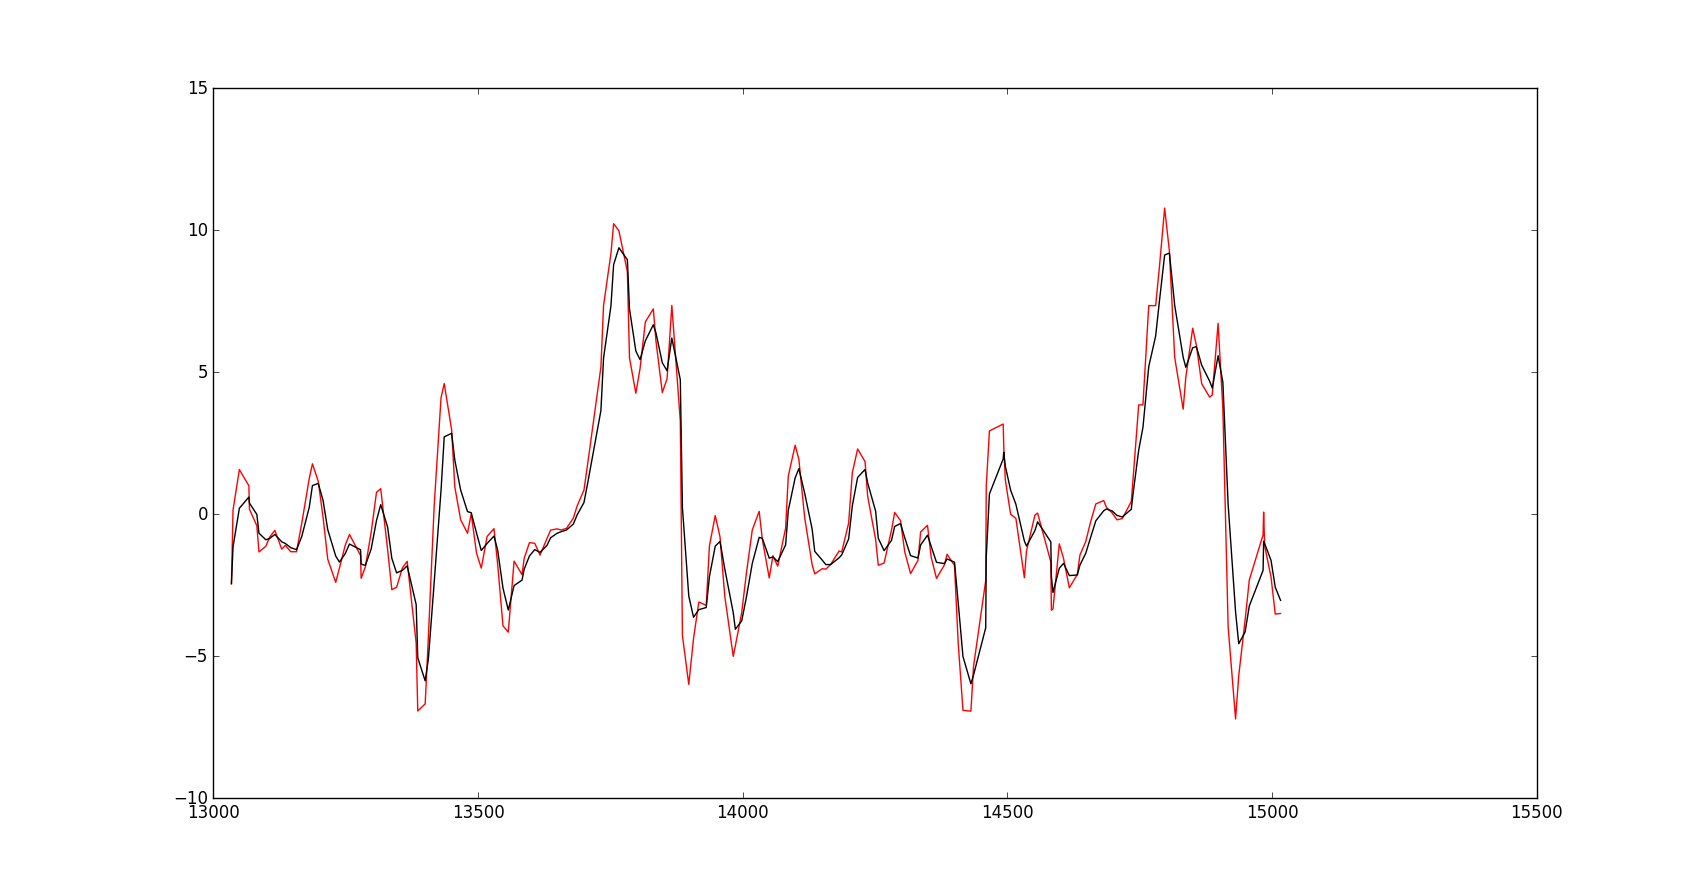
\includegraphics[scale=0.3]{pictures/LOWPASSfiltereddata.png}}
\caption{Raw z-axis(red) readings vs low-pass filtered(black) data.}
\end{figure}


\section{Smoothing}
There being various method of smoothing, moving average was selected for our analysis, as it smooths the graph while maintaining the characteristic of the graph. \newline

After many iterations the window size of 5 was chosen, if a large value of window size had been used then the variations could have not been so obvious. After experimenting it was also found out that running moving average 3-5 times with small window size proved to be better than running 1-2 window average with large window size as the gait cycle period points are short. \newline


The average of window size of data points are taken as average and the value is set to the median element. The weight given to every points in the window size over summation is the same.\newline
$$X_\frac{m+n}{2} = \frac{X_m + X_{m+1}+ \cdots + X_n}{n-m+1}
      = \frac{1}{n-m+1}\sum_{i=m}^{n} X_i \ \ \ \cite{movingaverage}$$

\begin{figure}
\center{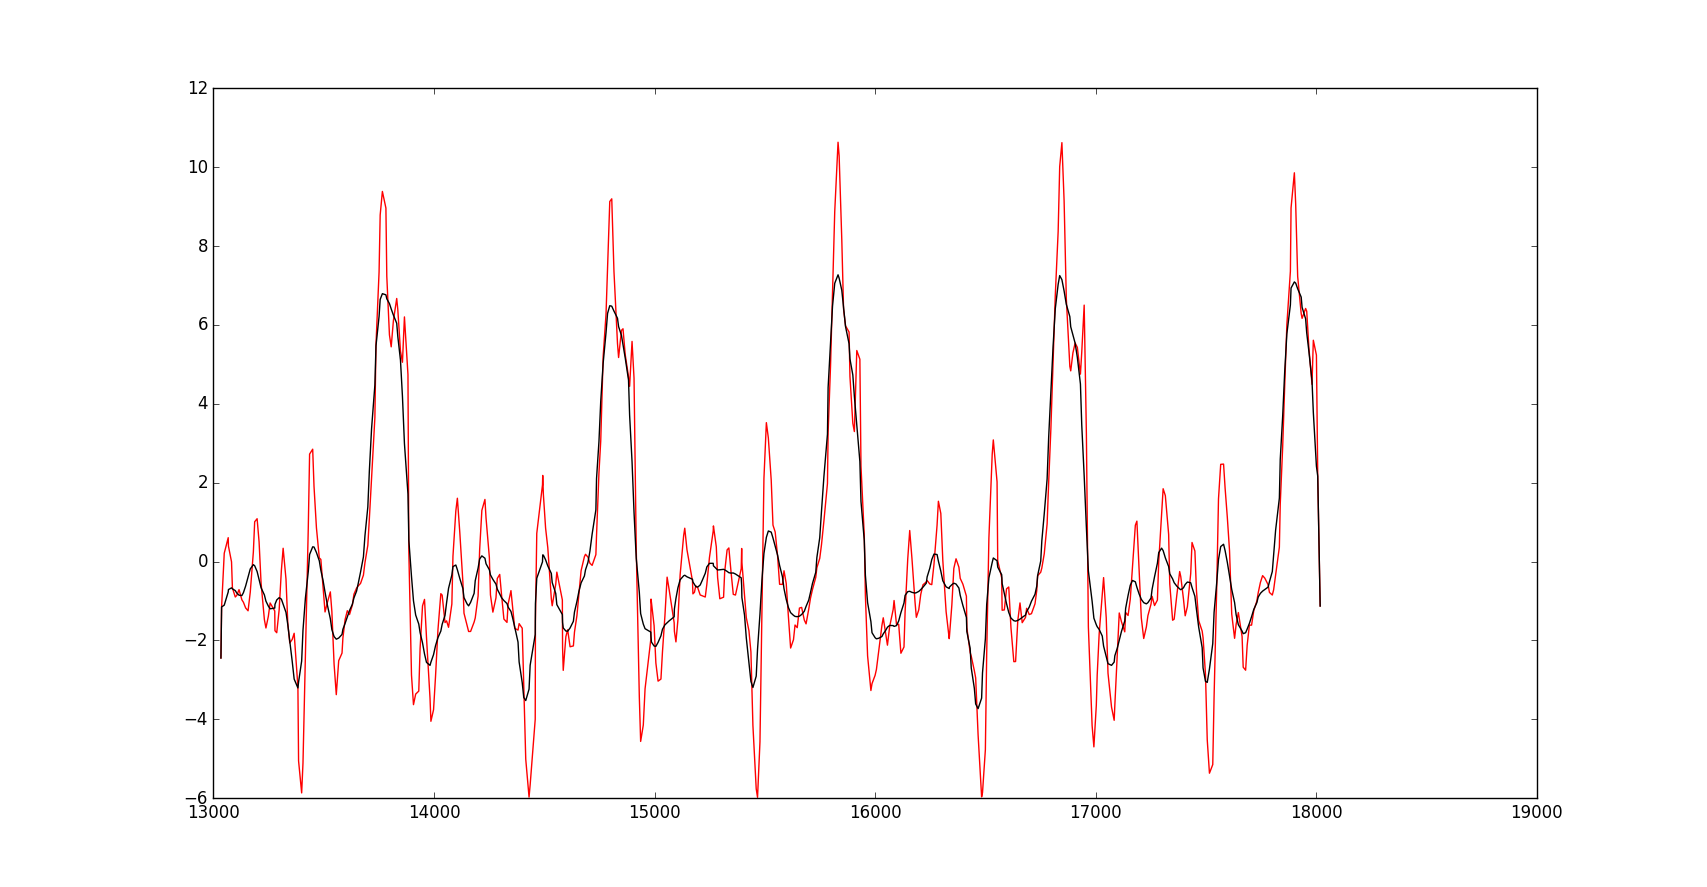
\includegraphics[scale=0.3]{pictures/maax3.png}}
\caption{Moving Average applied on low-pass filtered data.}
\end{figure}

\section{Normalization}

Data is then normalized to reduce the distance between the maximum and minimum of 
gait cycle points while preserving the characteristics of the graph.\newline

$$ y_{i} = \frac{x_{i} - min(x)}{max(x) - min(x)} \ \ \ \cite{normal} $$
\begin{figure}
\center{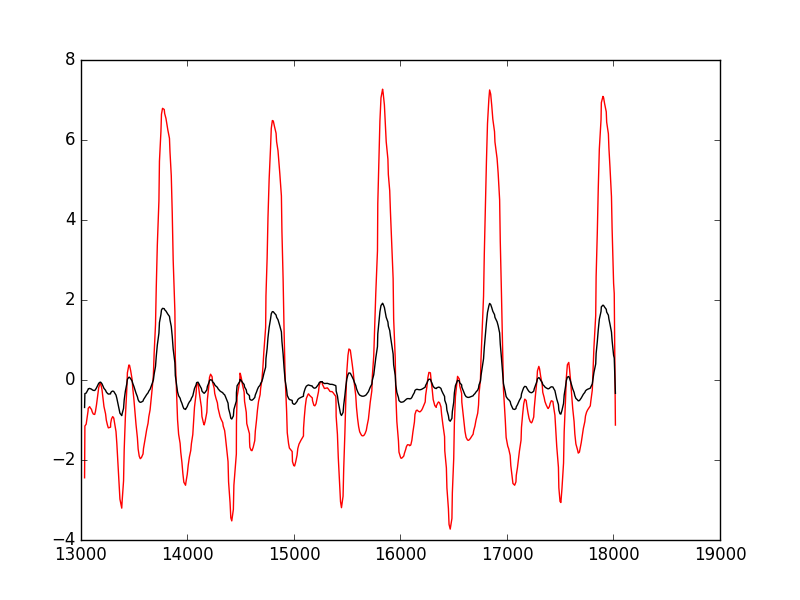
\includegraphics[scale=0.6]{pictures/normalized.png}}
\caption{Normalization done on moving averaged data.}
\end{figure}

